% Editable native annotations around unchanged verified IDE photographs.
\par
\begin{figure}[htbp]
  \centering
  \newsavebox{\MARSfirclippedregistersBox}
  \sbox{\MARSfirclippedregistersBox}{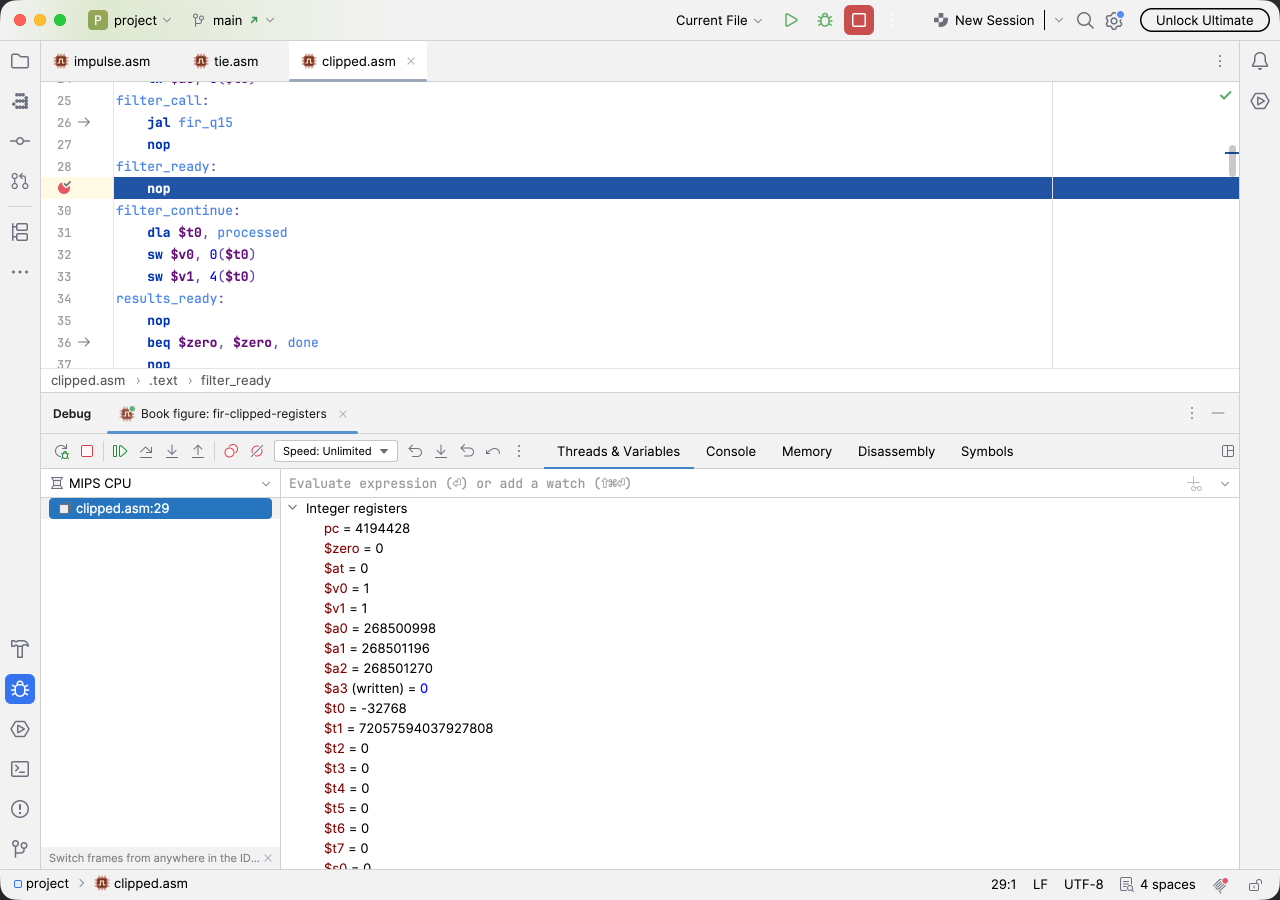
\includegraphics[artifact]{packages/021-fixed-point-fir/captures/f04/registers.png}}
  \newsavebox{\MARSfirclippedinputBox}
  \sbox{\MARSfirclippedinputBox}{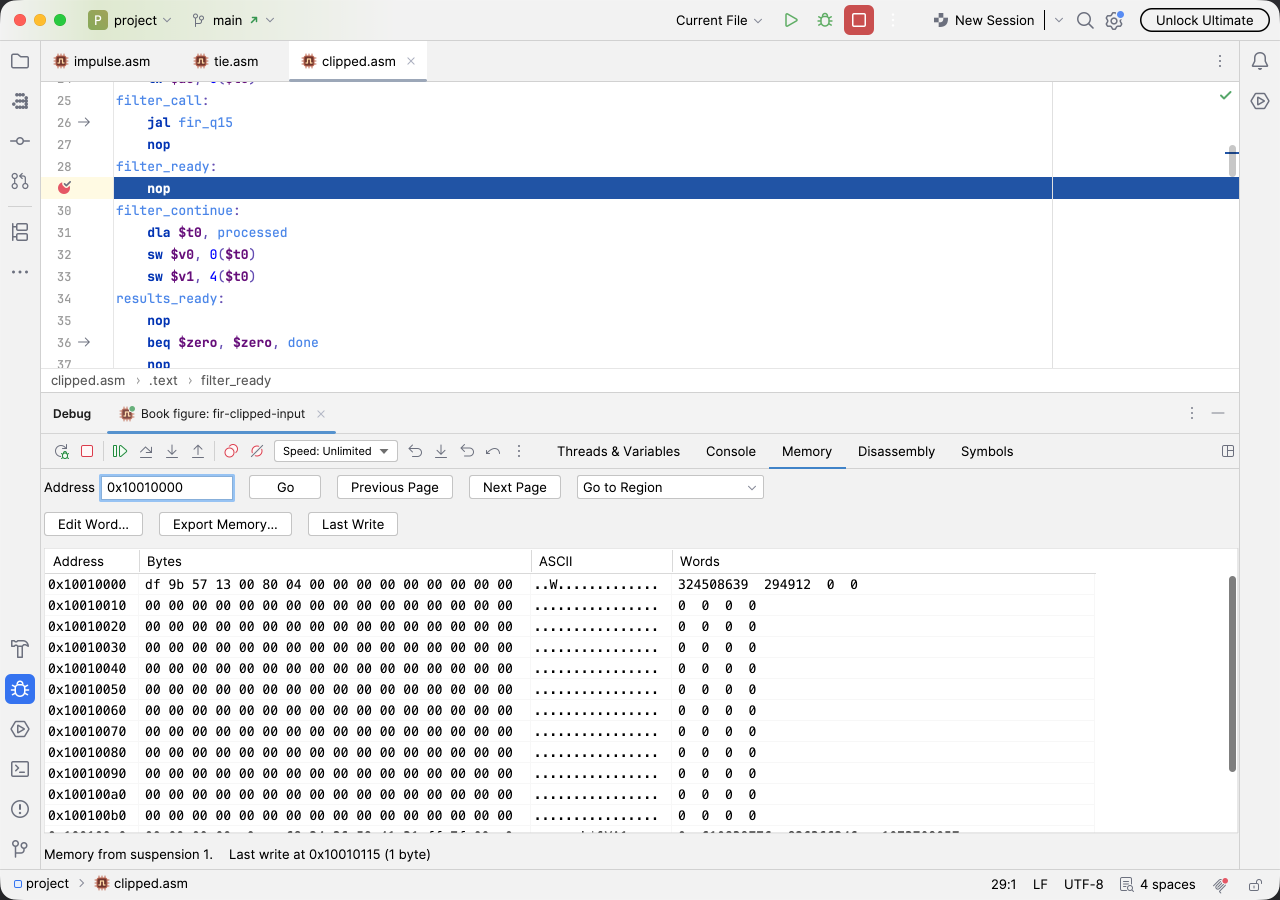
\includegraphics[artifact]{packages/021-fixed-point-fir/captures/f04/input.png}}
  \newsavebox{\MARSfirclippedcoefficientsBox}
  \sbox{\MARSfirclippedcoefficientsBox}{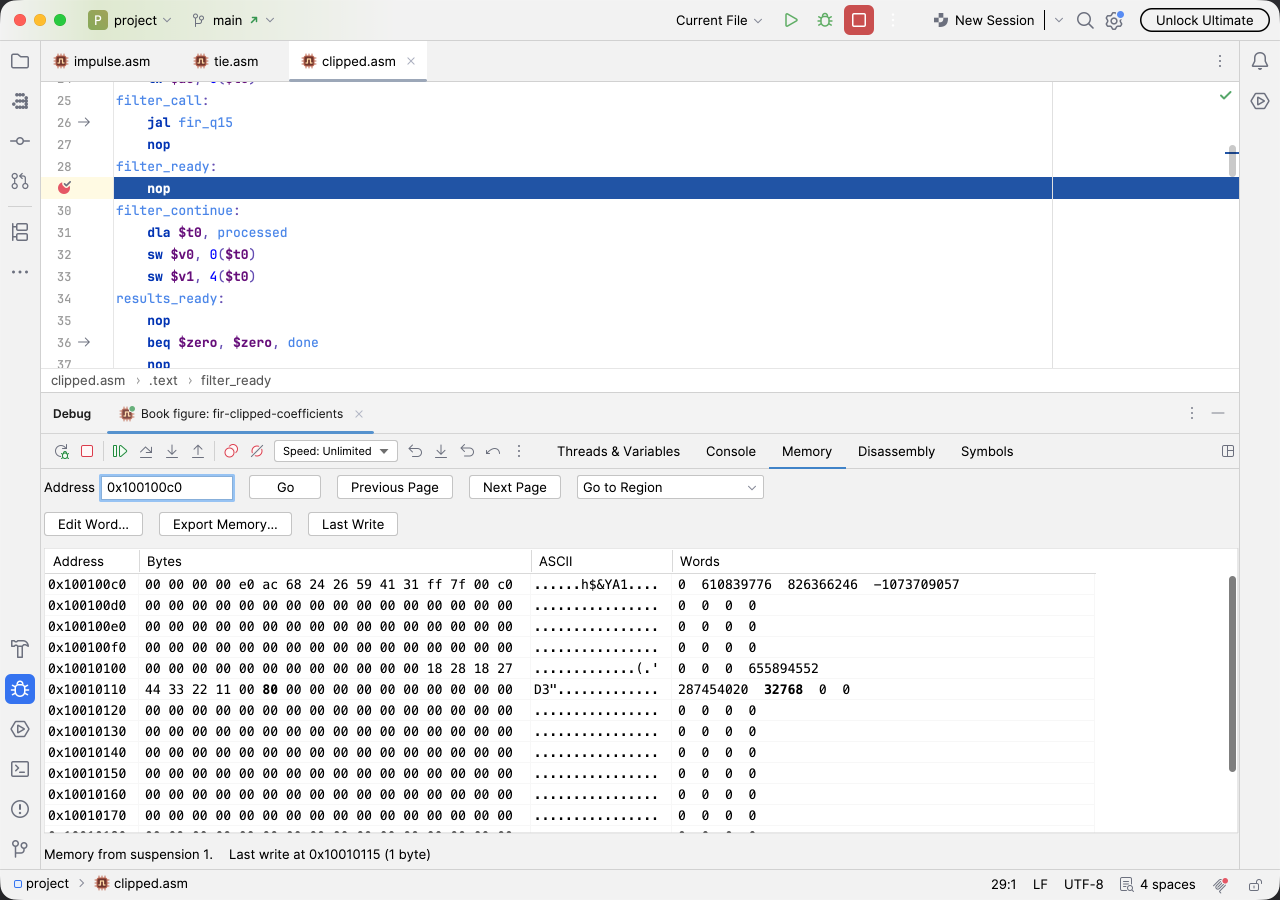
\includegraphics[artifact]{packages/021-fixed-point-fir/captures/f04/coefficients.png}}
  \newsavebox{\MARSfirclippedoutputBox}
  \sbox{\MARSfirclippedoutputBox}{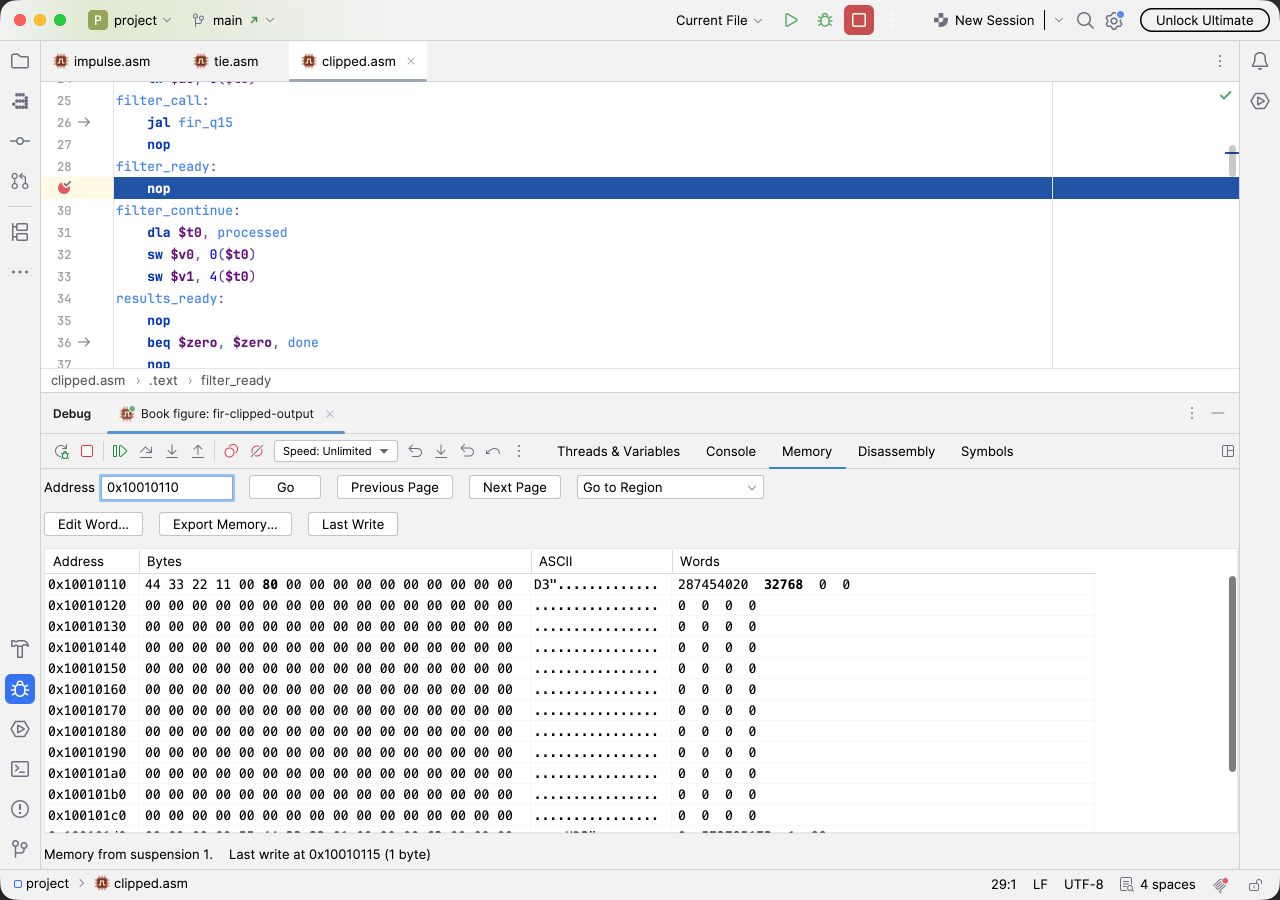
\includegraphics[artifact]{packages/021-fixed-point-fir/captures/f04/output.png}}
  \newsavebox{\MARSfirclippedcallerBox}
  \sbox{\MARSfirclippedcallerBox}{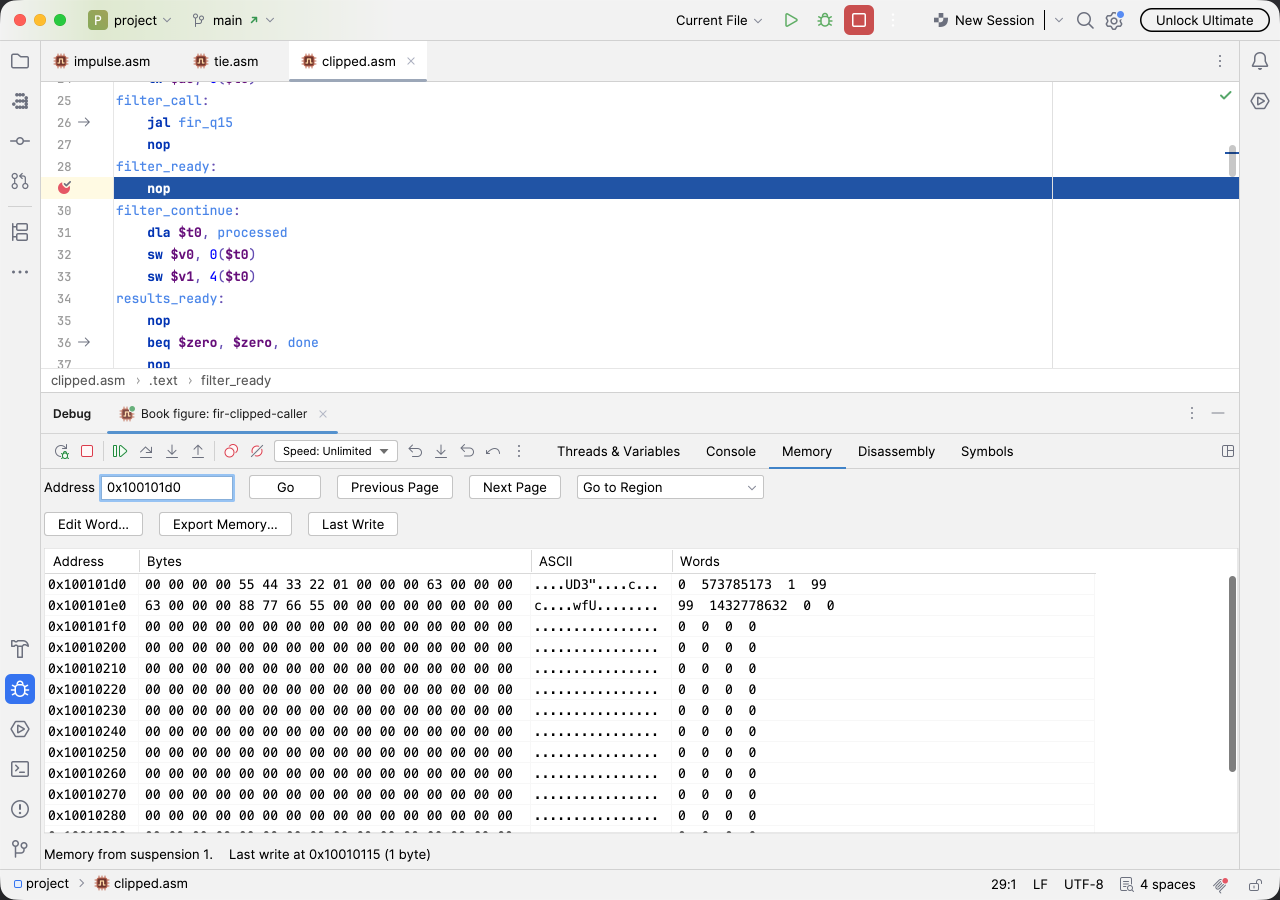
\includegraphics[artifact]{packages/021-fixed-point-fir/captures/f04/caller.png}}
  \edef\MARSfirclippedsourceLeft{\the\dimexpr0.036718750\wd\MARSfirclippedregistersBox\relax}
  \edef\MARSfirclippedsourceBottom{\the\dimexpr0.774444444\ht\MARSfirclippedregistersBox\relax}
  \edef\MARSfirclippedsourceRight{\the\dimexpr0.713281250\wd\MARSfirclippedregistersBox\relax}
  \edef\MARSfirclippedsourceTop{\the\dimexpr0.170000000\ht\MARSfirclippedregistersBox\relax}
  \edef\MARSfirclippedregistersLeft{\the\dimexpr0.246093750\wd\MARSfirclippedregistersBox\relax}
  \edef\MARSfirclippedregistersBottom{\the\dimexpr0.312222222\ht\MARSfirclippedregistersBox\relax}
  \edef\MARSfirclippedregistersRight{\the\dimexpr0.553906250\wd\MARSfirclippedregistersBox\relax}
  \edef\MARSfirclippedregistersTop{\the\dimexpr0.640000000\ht\MARSfirclippedregistersBox\relax}
  \edef\MARSfirclippedinputLeft{\the\dimexpr0.034375000\wd\MARSfirclippedinputBox\relax}
  \edef\MARSfirclippedinputBottom{\the\dimexpr0.311111111\ht\MARSfirclippedinputBox\relax}
  \edef\MARSfirclippedinputRight{\the\dimexpr0.584375000\wd\MARSfirclippedinputBox\relax}
  \edef\MARSfirclippedinputTop{\the\dimexpr0.608888889\ht\MARSfirclippedinputBox\relax}
  \edef\MARSfirclippedcoefficientsLeft{\the\dimexpr0.034375000\wd\MARSfirclippedcoefficientsBox\relax}
  \edef\MARSfirclippedcoefficientsBottom{\the\dimexpr0.311111111\ht\MARSfirclippedcoefficientsBox\relax}
  \edef\MARSfirclippedcoefficientsRight{\the\dimexpr0.584375000\wd\MARSfirclippedcoefficientsBox\relax}
  \edef\MARSfirclippedcoefficientsTop{\the\dimexpr0.608888889\ht\MARSfirclippedcoefficientsBox\relax}
  \edef\MARSfirclippedoutputLeft{\the\dimexpr0.034375000\wd\MARSfirclippedoutputBox\relax}
  \edef\MARSfirclippedoutputBottom{\the\dimexpr0.334444444\ht\MARSfirclippedoutputBox\relax}
  \edef\MARSfirclippedoutputRight{\the\dimexpr0.584375000\wd\MARSfirclippedoutputBox\relax}
  \edef\MARSfirclippedoutputTop{\the\dimexpr0.608888889\ht\MARSfirclippedoutputBox\relax}
  \edef\MARSfirclippedcallerLeft{\the\dimexpr0.034375000\wd\MARSfirclippedcallerBox\relax}
  \edef\MARSfirclippedcallerBottom{\the\dimexpr0.311111111\ht\MARSfirclippedcallerBox\relax}
  \edef\MARSfirclippedcallerRight{\the\dimexpr0.584375000\wd\MARSfirclippedcallerBox\relax}
  \edef\MARSfirclippedcallerTop{\the\dimexpr0.608888889\ht\MARSfirclippedcallerBox\relax}
  \begin{tikzpicture}[alt={Six annotated panels at filter_ready show one output and one clipped. The second input is four instead of three, with unchanged coefficients 32767 and minus 16384. The exact accumulator is minus 1073774592 and its rounded value is minus 32769, so saturation stores minus 32768. The output bytes still match the un-clipped tie case, but v1 is one.}]
    \node[anchor=north west,inner sep=0,font=\small\bfseries] (source-title) at (6mm,0) {Next instruction at this boundary};
    \node[anchor=north west,inner sep=0] (source) at ([yshift=-1mm]source-title.south west) {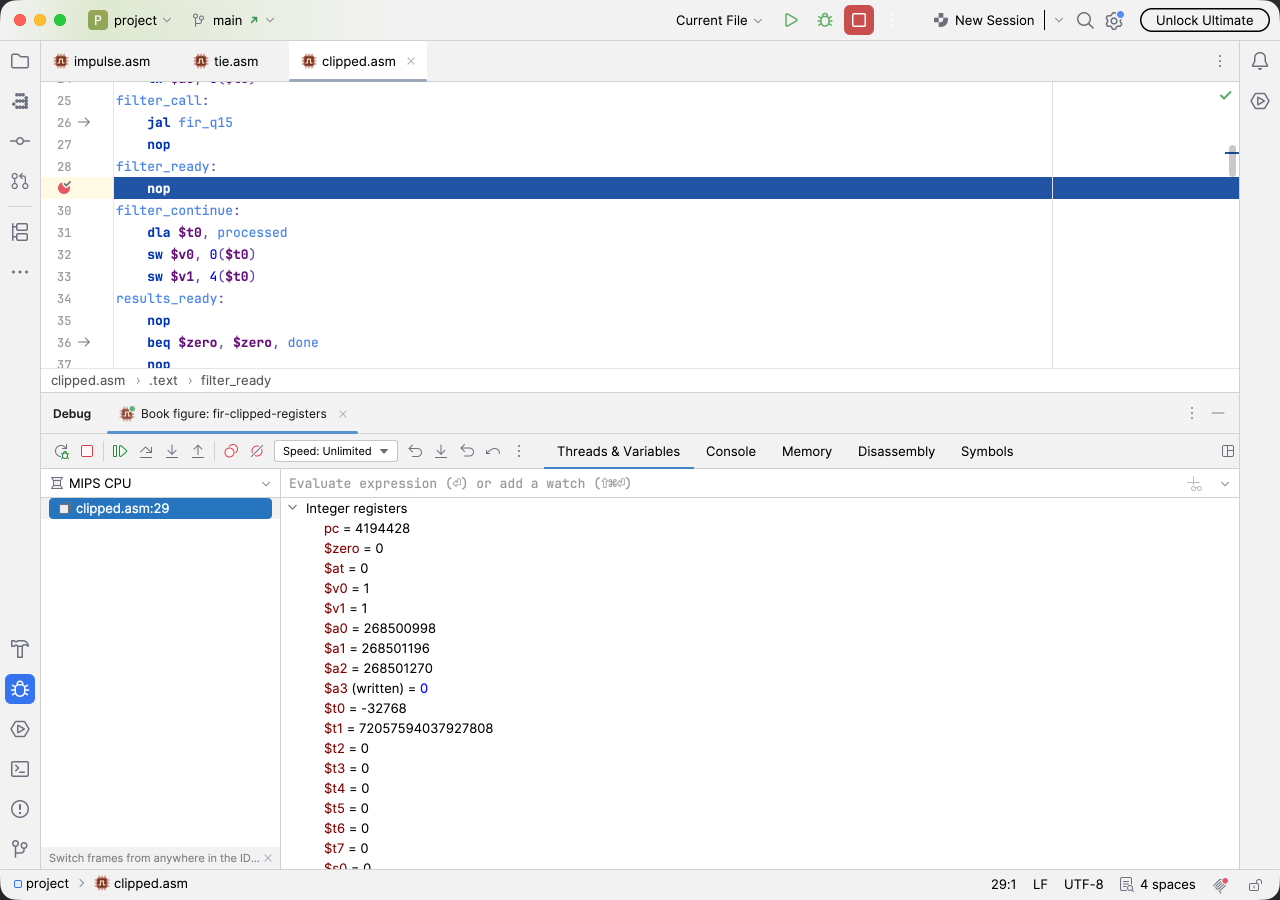
\includegraphics[width=0.54\linewidth,artifact,trim={\MARSfirclippedsourceLeft{} \MARSfirclippedsourceBottom{} \MARSfirclippedsourceRight{} \MARSfirclippedsourceTop{}},clip]{packages/021-fixed-point-fir/captures/f04/registers.png}};
    \begin{scope}[shift={(source.south west)},x={($(source.south east)-(source.south west)$)},y={($(source.north west)-(source.south west)$)}]
      \draw[black,line width=0.7pt] (0.215625000,0.080000000) rectangle (0.384375000,0.520000000);
      \node[draw=black,fill=white,circle,inner sep=1.5pt,font=\footnotesize] at ($(0.215625000,0.520000000)+(-3mm,0)$) {1};
    \end{scope}
    \node[anchor=north west,inner sep=0,font=\small\bfseries] (registers-title) at (0.58\linewidth,0 |- source-title.north) {Register values at this boundary};
    \node[anchor=north west,inner sep=0] (registers) at ([yshift=-1mm]registers-title.south west) {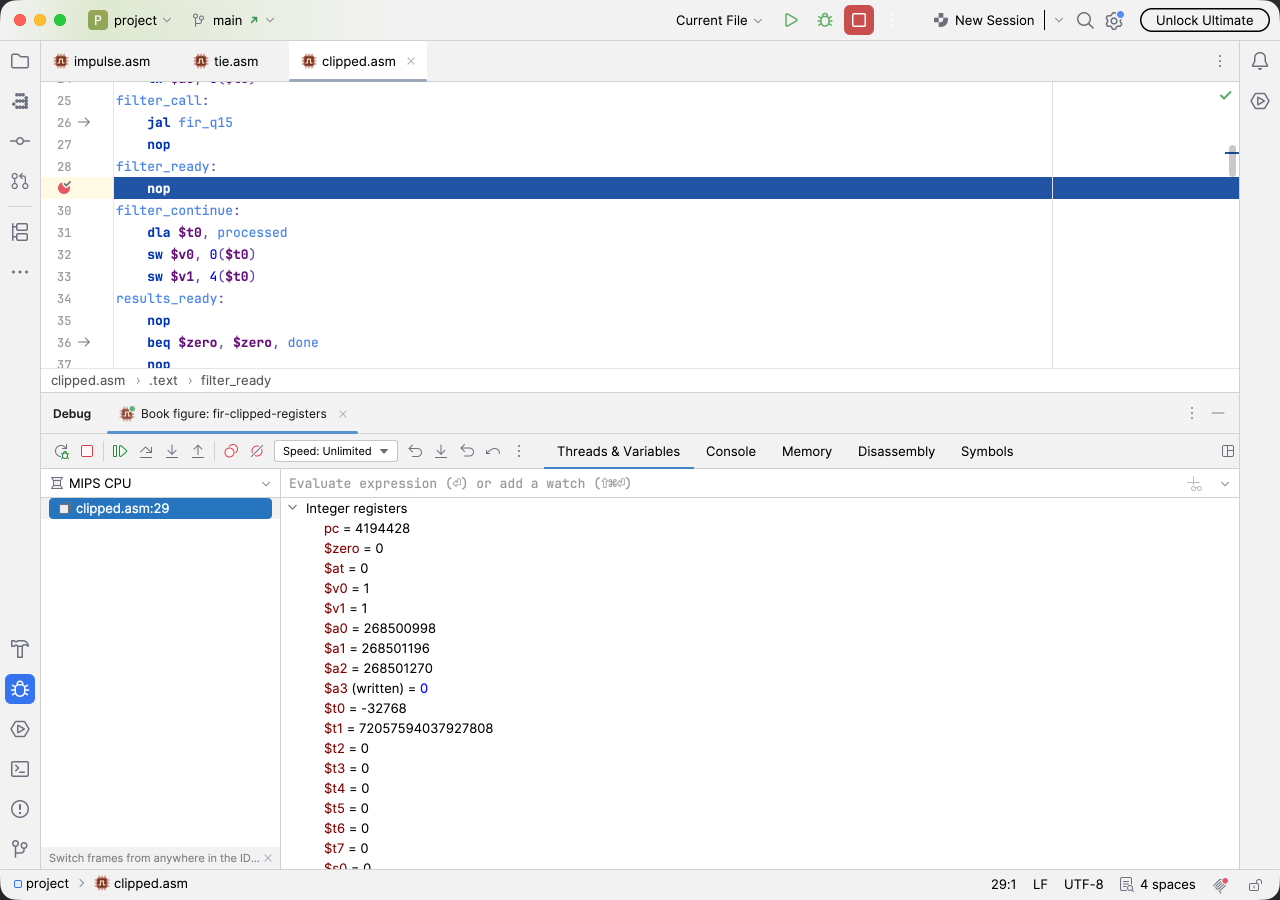
\includegraphics[width=0.42\linewidth,artifact,trim={\MARSfirclippedregistersLeft{} \MARSfirclippedregistersBottom{} \MARSfirclippedregistersRight{} \MARSfirclippedregistersTop{}},clip]{packages/021-fixed-point-fir/captures/f04/registers.png}};
    \begin{scope}[shift={(registers.south west)},x={($(registers.south east)-(registers.south west)$)},y={($(registers.north west)-(registers.south west)$)}]
      \draw[black,line width=0.7pt] (0.023437500,0.023255814) rectangle (0.218750000,0.953488372);
      \node[draw=black,fill=white,circle,inner sep=1.5pt,font=\footnotesize] at ($(0.023437500,0.953488372)+(-3mm,0)$) {2};
    \end{scope}
    \node[anchor=north west,inner sep=0,font=\small\bfseries] (input-title) at ([yshift=-1mm]source.south west) {Input window detail};
    \node[anchor=north west,inner sep=0] (input) at ([yshift=-1mm]input-title.south west) {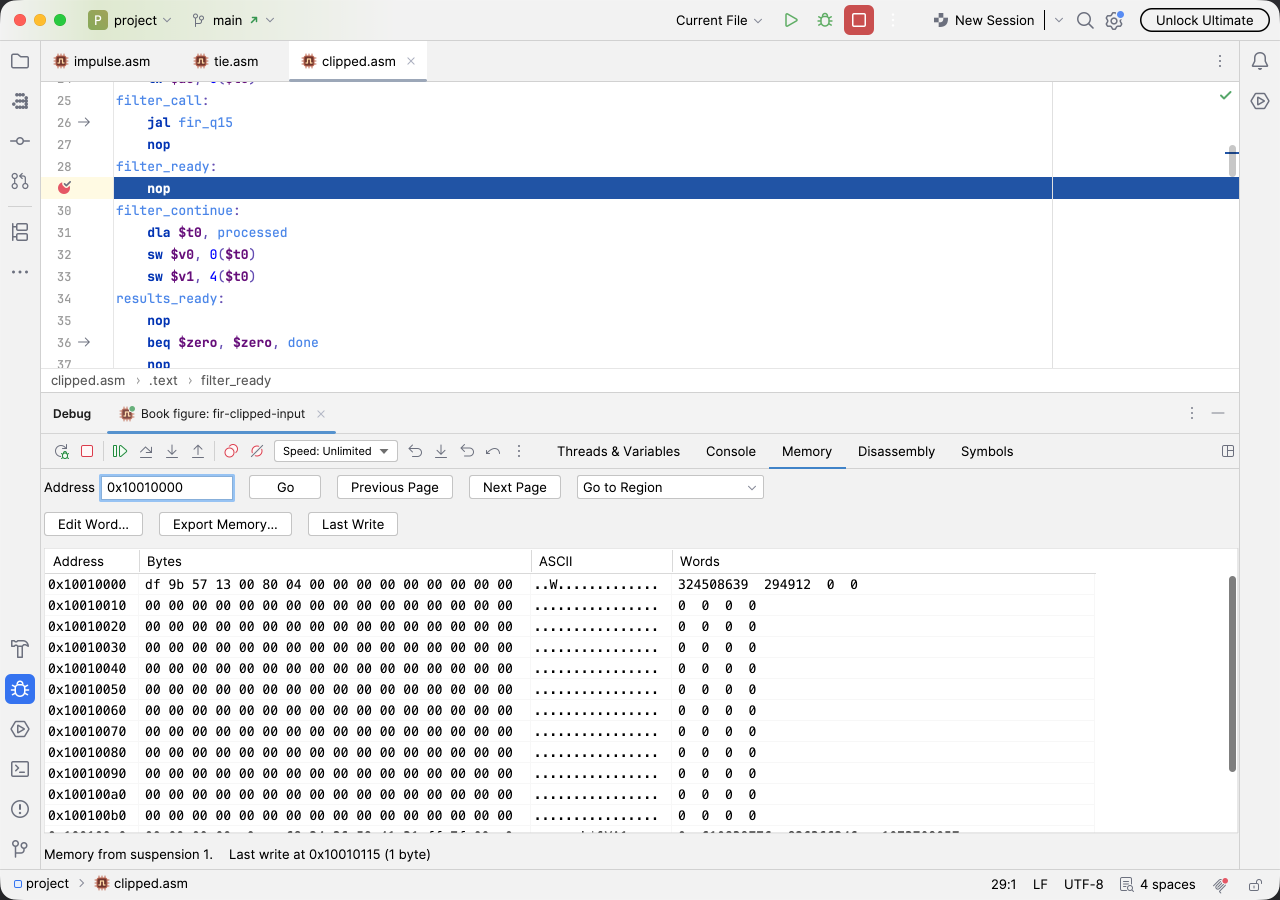
\includegraphics[width=0.84\linewidth,artifact,trim={\MARSfirclippedinputLeft{} \MARSfirclippedinputBottom{} \MARSfirclippedinputRight{} \MARSfirclippedinputTop{}},clip]{packages/021-fixed-point-fir/captures/f04/input.png}};
    \begin{scope}[shift={(input.south west)},x={($(input.south east)-(input.south west)$)},y={($(input.north west)-(input.south west)$)}]
      \draw[black,line width=0.7pt] (0.194672131,0.055555556) rectangle (0.997950820,0.638888889);
      \node[draw=black,fill=white,circle,inner sep=1.5pt,font=\footnotesize] at ($(0,0.638888889)+(-3mm,0)$) {3};
    \end{scope}
    \node[anchor=north west,inner sep=0,font=\small\bfseries] (coefficients-title) at ([yshift=-1mm]input.south west) {Eight signed coefficient codes};
    \node[anchor=north west,inner sep=0] (coefficients) at ([yshift=-1mm]coefficients-title.south west) {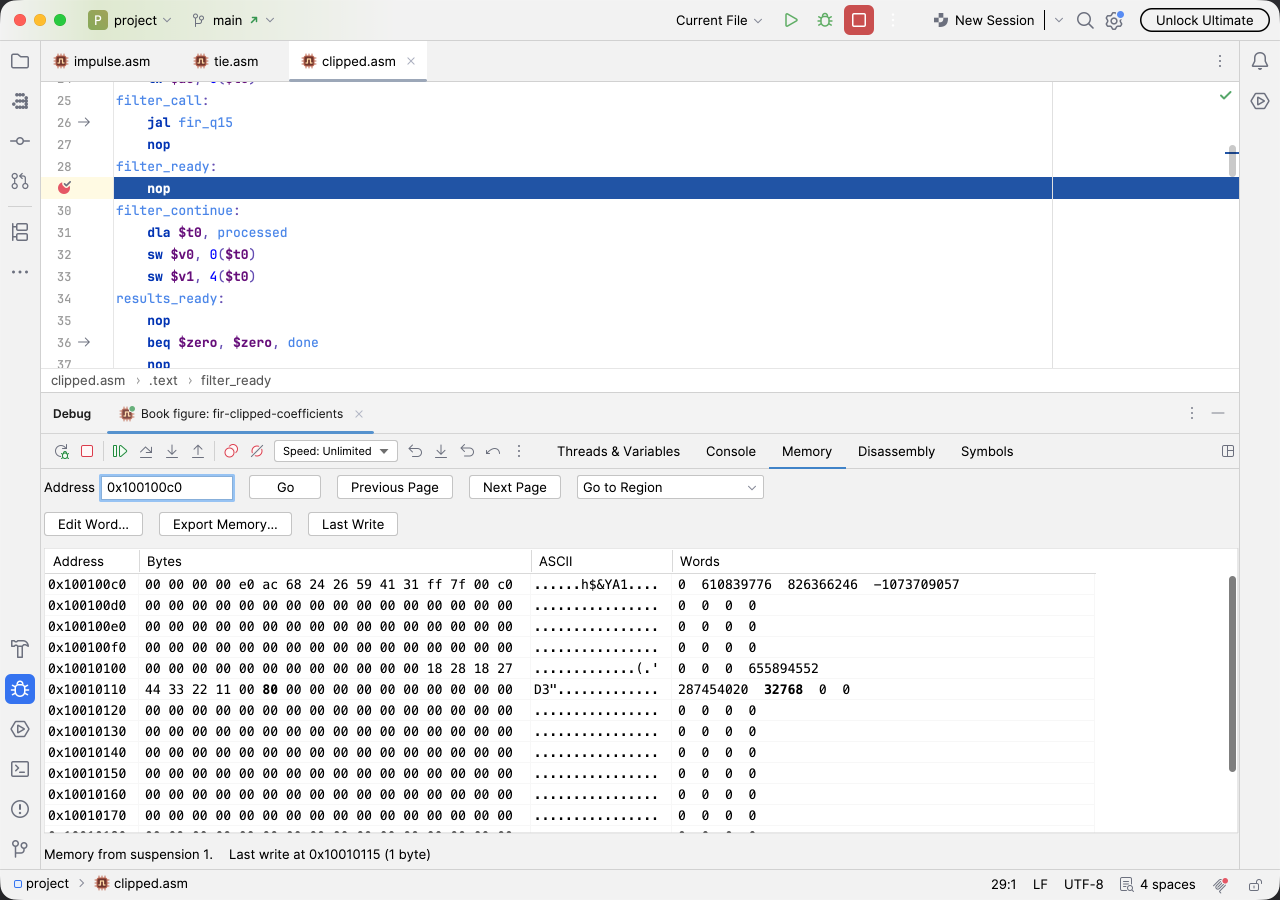
\includegraphics[width=0.84\linewidth,artifact,trim={\MARSfirclippedcoefficientsLeft{} \MARSfirclippedcoefficientsBottom{} \MARSfirclippedcoefficientsRight{} \MARSfirclippedcoefficientsTop{}},clip]{packages/021-fixed-point-fir/captures/f04/coefficients.png}};
    \begin{scope}[shift={(coefficients.south west)},x={($(coefficients.south east)-(coefficients.south west)$)},y={($(coefficients.north west)-(coefficients.south west)$)}]
      \draw[black,line width=0.7pt] (0.194672131,0.055555556) rectangle (0.997950820,0.638888889);
      \node[draw=black,fill=white,circle,inner sep=1.5pt,font=\footnotesize] at ($(0,0.638888889)+(-3mm,0)$) {4};
    \end{scope}
    \node[anchor=north west,inner sep=0,font=\small\bfseries] (output-title) at ([yshift=-1mm]coefficients.south west) {Selected output halfwords};
    \node[anchor=north west,inner sep=0] (output) at ([yshift=-1mm]output-title.south west) {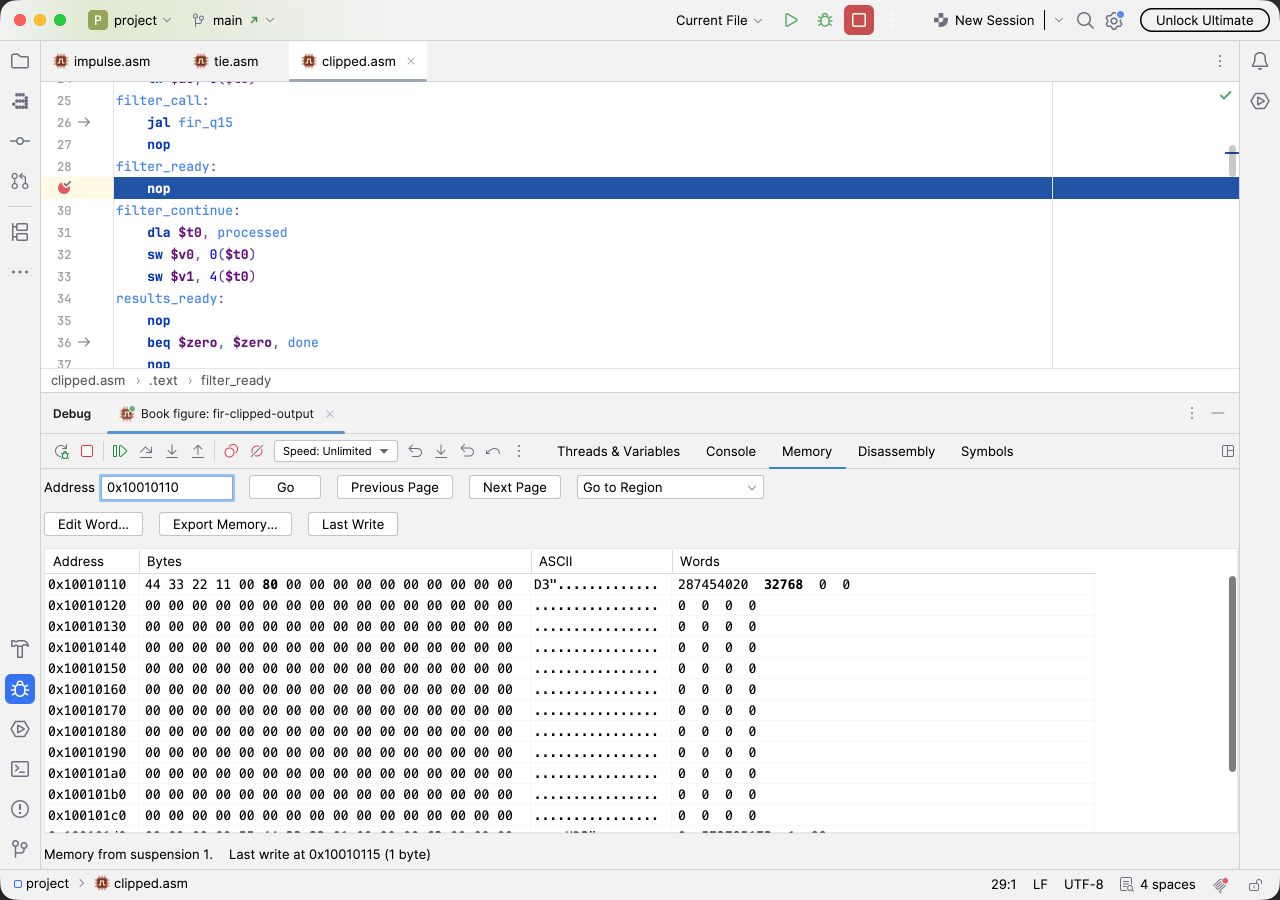
\includegraphics[width=0.84\linewidth,artifact,trim={\MARSfirclippedoutputLeft{} \MARSfirclippedoutputBottom{} \MARSfirclippedoutputRight{} \MARSfirclippedoutputTop{}},clip]{packages/021-fixed-point-fir/captures/f04/output.png}};
    \begin{scope}[shift={(output.south west)},x={($(output.south east)-(output.south west)$)},y={($(output.north west)-(output.south west)$)}]
      \draw[black,line width=0.7pt] (0.194672131,0.078431373) rectangle (0.997950820,0.490196078);
      \node[draw=black,fill=white,circle,inner sep=1.5pt,font=\footnotesize] at ($(0,0.490196078)+(-3mm,0)$) {5};
    \end{scope}
    \node[anchor=north west,inner sep=0,font=\small\bfseries] (caller-title) at ([yshift=-1mm]output.south west) {Count and saved caller results};
    \node[anchor=north west,inner sep=0] (caller) at ([yshift=-1mm]caller-title.south west) {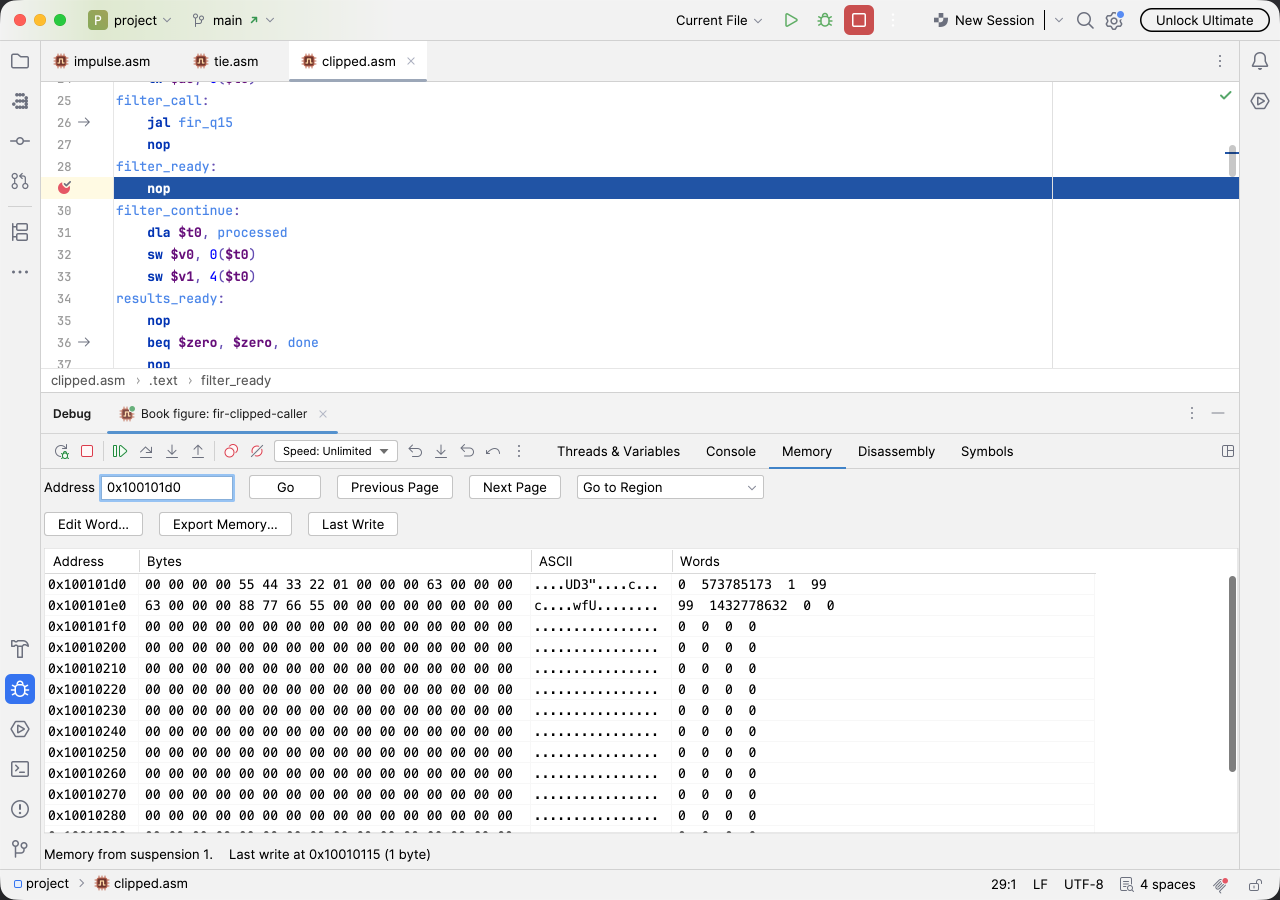
\includegraphics[width=0.84\linewidth,artifact,trim={\MARSfirclippedcallerLeft{} \MARSfirclippedcallerBottom{} \MARSfirclippedcallerRight{} \MARSfirclippedcallerTop{}},clip]{packages/021-fixed-point-fir/captures/f04/caller.png}};
    \begin{scope}[shift={(caller.south west)},x={($(caller.south east)-(caller.south west)$)},y={($(caller.north west)-(caller.south west)$)}]
      \draw[black,line width=0.7pt] (0.194672131,0.055555556) rectangle (0.997950820,0.638888889);
      \node[draw=black,fill=white,circle,inner sep=1.5pt,font=\footnotesize] at ($(0,0.638888889)+(-3mm,0)$) {6};
    \end{scope}
  \end{tikzpicture}
  \par\smallskip
  \begin{minipage}{\linewidth}
    \small
    \begin{enumerate}
      \setlength{\itemsep}{2pt}
            \setlength{\parsep}{0pt}
      \item This fixture changes the second input from 3 to 4 and keeps the same one-output count, coefficients and observation boundary. The function has completed; caller result publication remains ahead.
      \item \texttt{\$v0 = 1} and \texttt{\$v1 = 1}. The rounded integer is below the minimum signed halfword, so saturation contributes one clipping event.
      \item Input begins with $-32768$ and 4, followed by six zeros. The changed halfword is \texttt{04 00}. A one-code input change alters its product by $-16384$ because that tap\textquotesingle s coefficient is $-16384$.
      \item The coefficient array is unchanged. The exact accumulator becomes $-1073774592$, giving a rounded integer of $-32769$. Saturation then selects $-32768$. Rounding and the range check are separate operations in that order.
      \item The output at \texttt{0x10010114} is again \texttt{00 80}. These bytes match the preceding halfway fixture, although the clipping counts differ. Compare the rounded value and \texttt{v1} when deciding how the endpoint was produced.
      \item Count is 1 and the saved results are still 99. Continuing will publish processed 1 and clipped 1. Input, coefficients, guards and every output byte outside the selected halfword remain unchanged.
    \end{enumerate}
  \end{minipage}
  \caption{Changing one input code produces the same endpoint with one clipping event.}
  \label{capture:021-fixed-point-fir-f04}
  \label{fir-f04}
\end{figure}
\par
